\documentclass[tikz,border=6pt]{standalone}
\usepackage{amsmath,amssymb,mathtools,physics,bm,nicefrac,wasysym}
\usepackage{xcolor}

\definecolor{colone}{RGB}{180,60,60}
\definecolor{coltwo}{RGB}{60,110,180}
\definecolor{colthree}{RGB}{60,140,80}

\definecolor{accent}{HTML}{A13D2C}
\definecolor{accent2}{HTML}{2B5F6B}
\definecolor{muted}{HTML}{5A564F}
\definecolor{panel}{HTML}{F8F6F0}
\definecolor{linecol}{HTML}{D8D2C4}
\definecolor{ink}{HTML}{1E1C1A}
\definecolor{astroblue}{HTML}{1B4F72}
\definecolor{astrodark}{HTML}{17202A}
\definecolor{sunyellow}{HTML}{E8A33D}

\usetikzlibrary{calc,arrows.meta,positioning,decorations.pathreplacing,decorations.markings,angles,quotes,shapes.geometric}
\usepackage{tikz-3dplot}

\newcommand{\vecr}{\vec r}
\newcommand{\vecL}{\vec L}
\newcommand{\vecA}{\vec A}
\newcommand{\vecf}{\vec f}
\newcommand{\vecF}{\vec F}
\newcommand{\vecp}{\vec p}
\newcommand{\avg}[1]{\left\langle #1\right\rangle}
\newcommand{\vecx}{\vec x}
\newcommand{\hatn}{\hat n}
\newcommand{\rhat}{\hat r}
\newcommand{\phihat}{\hat\phi}
\newcommand{\thetahat}{\hat\theta}
\newcommand{\note}[1]{\textcolor{blue!60!black}{\textit{[#1]}}}

% Astronomical acronyms
\newcommand{\LST}{\mathrm{LST}}
\newcommand{\GST}{\mathrm{GST}}
\newcommand{\GMST}{\mathrm{GMST}}
\newcommand{\GAST}{\mathrm{GAST}}
\newcommand{\LMST}{\mathrm{LMST}}
\newcommand{\LAST}{\mathrm{LAST}}
\newcommand{\UT}{\mathrm{UT}}
\newcommand{\UTC}{\mathrm{UTC}}
\newcommand{\TAI}{\mathrm{TAI}}
\newcommand{\TT}{\mathrm{TT}}
\newcommand{\TDB}{\mathrm{TDB}}
\newcommand{\JD}{\mathrm{JD}}
\newcommand{\MJD}{\mathrm{MJD}}
\newcommand{\EoT}{\mathrm{EoT}}
\newcommand{\SNR}{\mathrm{SNR}}
\newcommand{\RON}{\mathrm{RON}}

% Helper commands for specific diagrams
\newcommand{\midlinelabel}[3]{
    \node (midlabel) at ($ (#1)!.5!(#2) $) {#3};
    \draw[stealth-] (#1) --  (midlabel);
    \draw[-stealth] (midlabel) -- (#2);
}
\newcommand{\midlinelabell}[3]{
    \node[fill = white, inner sep = 0.2pt, outer sep=3pt] (midlabel) at ($ (#1)!.5!(#2) $) {#3};
    \draw[stealth-] (#1) --  (midlabel);
    \draw[-stealth] (midlabel) -- (#2);
}
\newcommand{\midlinelabelll}[3]{
    \node[fill = white, inner sep = 0.2pt, outer sep=3pt,scale=0.6] (midlabel) at ($ (#1)!.5!(#2) $) {#3};
    \draw[stealth-] (#1) --  (midlabel);
    \draw[-stealth] (midlabel) -- (#2);
}



\begin{document}
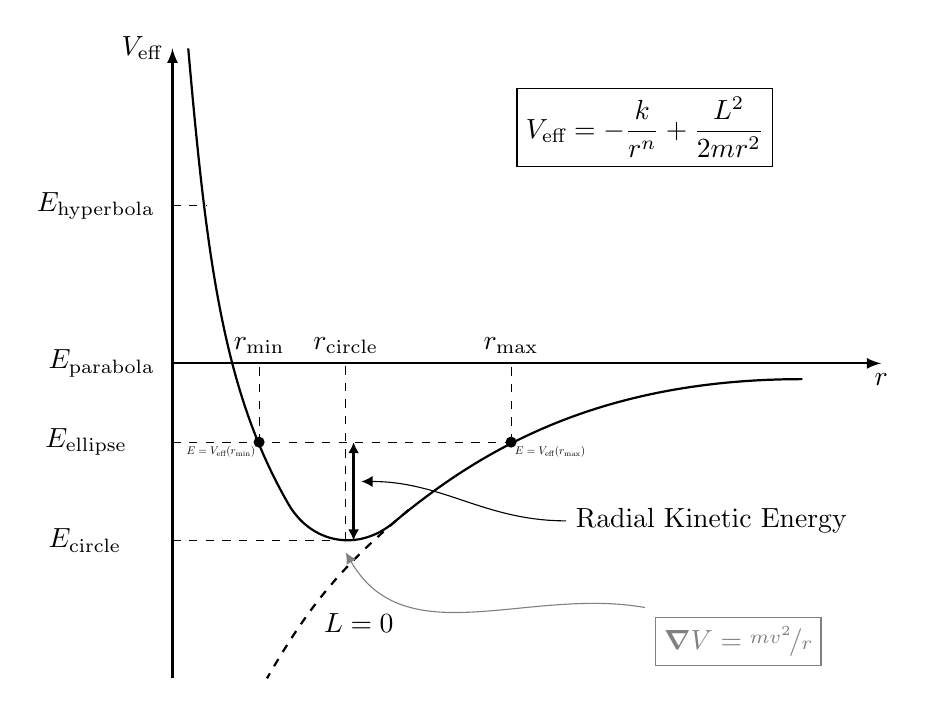
\begin{tikzpicture}[>={Latex[length=4,width=4]}]
		% Axis
		\draw[-latex, thick] (0,-1) -- (0,7) node[left] {$V_{\text{eff}}$};
		\draw[-latex, thick] (0,3) -- (9,3) node[below] {$r$};
		\draw[rounded corners=30,thick] (8,2.8) to[out=180,in=40] (2,0.3) to[out=120,in=-85] (0.2,7) ;
		\draw[dashed,rounded corners=30,thick] (3,1.14) to[out=220,in=60] (1.2,-1);
		\node[anchor=east, xshift=-3pt] at (0,3) {$E_{\text{parabola}}$};
		\draw[dashed] (0,0.75)--(2.2,0.75);
		\node[anchor=east, xshift=-15pt] at (0,0.75) {$E_{\text{circle}}$};
		\draw[<-,gray] (2.2,0.6)  to[out=-60,in=170](6,-0.1)node[below right]{$\boxed{\grad{V}=\nicefrac{mv^2}{r}}$};
		\draw[dashed] (0,2)--(4.25,2);
		\node[anchor=east, xshift=-13pt] at (0,2) {$E_{\text{ellipse}}$};
		\draw[dashed] (0,5)--(0.425,5);
		\node[anchor=east, xshift=-3pt] at (0,5) {$E_{\text{hyperbola}}$};
		\draw[dashed] (2.2,.75)--(2.2,3);
		\node[above] at (2.2,3) {$r_{\text{circle}}$};
		\draw[dashed] (1.1,2)--(1.1,3);
		\node[above] at (1.1,3) {$r_{\text{min}}$};
		\fill (1.1,2) circle (2pt) node[below left,scale=0.4] {$E=V_{\text{eff}}(r_{\text{min}})$};
		\draw[dashed] (4.3,2)--(4.3,3);
		\fill (4.3,2) circle (2pt) node[below right,scale=0.4] {$E=V_{\text{eff}}(r_{\text{max}})$};
		\node[above] at (4.3,3) {$r_{\text{max}}$};
		\node[right] at (1.8,-0.3) {$L=0$};
		\draw[<->,thick] (2.3,0.75)--(2.3,2);
		\draw[<-] (2.4,1.5) to[out=0,in=180] (5,1) node[right] {Radial Kinetic Energy};
		\node at (6,6) {$\boxed{V_{\text{eff}}=-\frac{k}{r^n}+\frac{L^2}{2mr^2}}$};
	\end{tikzpicture}
\end{document}
